%+----------------------------------------------------------------------------+
%| SLIDES: short presentation on my paper 1805.01696
%| Author: Antonio miti
%| Credit: Picture https://commons.wikimedia.org/wiki/File:Displacement_of_a_continuum.svg 
%| 			
%+----------------------------------------------------------------------------+


%- HandOut Flag -----------------------------------------------------------------------------------------
\newif\ifHandout
	\Handouttrue  %uncomment for the printable version


%- D0cum3nt ----------------------------------------------------------------------------------------------
\ifHandout
	\documentclass[handout,10pt]{beamer}   
	\setbeameroption{show notes} %print notes    
\else
	\documentclass[10pt]{beamer}
\fi


%- Packages ----------------------------------------------------------------------------------------------
\usepackage{verbatim}
\usepackage{appendixnumberbeamer}
\usepackage[mode=buildnew,subpreambles=true]{standalone}
\usepackage{amsmath, amssymb}
\usepackage{tikz}
\usetikzlibrary{arrows,shapes,snakes,calc}
\usetikzlibrary{shapes.callouts}
\usepackage{tikz-cd}
\usepackage{graphicx, animate}
\usepackage{hyperref}
\usepackage[english]{babel}
\usepackage{csquotes}



%--Beamer Style-----------------------------------------------------------------------------------------------
\usetheme{toninus}

%- T1tle P4g3 -------------------------------------------------------------------------------------------
\title{Homotopy co-momentum Map in Hydrodynamics} 
\subtitle{(Based on \href{http://arxiv.org/abs/1805.01696}{Arxiv:1805.01696})}
\author[AMM]{\href{https://dmf.unicatt.it/miti/}{Antonio Michele Miti}\\(Joint work with Mauro Spera)}
\institute[UCSC and KU Leuven]{
  \begin{tabular}[h]{ccc}
      Università Cattolica del Sacro Cuore & & KU Leuven \\
      Brescia, Italy & & Leuven, Belgium \\
      \href{https://dipartimenti.unicatt.it/dmf-home?rdeLocaleAttr=it}{
\includegraphics[width=3.5cm]{Logos/UnicattBS-logo}} & & 
      \href{https://wis.kuleuven.be/english}{
\includegraphics[width=4cm]{Logos/KULeuven_logo}}
  \end{tabular}      
}
\date[KULeuven_18] % (optional, should be abbreviation of conference name)
{	%(partly joint with: M.Spera)\\ 
	\href{http://www.uc.pt/en/congressos/13yrw}{13th International Young Researchers Workshop on Geometry, Mechanics and Control} \\
	{\vskip 1ex}
	Coimbra, December 6-8, 2018
}


%- WorkAround --------------------------------------------------------------------------------------------------------------
%Standalone with relative path
\newcommand{\includestandalonewithpath}[3][]
{
  \begingroup
  \newcommand{\datapath}{#2}
  \includestandalone[#1]{\datapath/#3}
  \endgroup
}

%Intermediate checkpoint slide
\newcommand{\checkpoint}[0]{
	\ifHandout

	\else
 	\begin{frame}{Outline}
  		%\tableofcontents[currentsection,currentsubsection]
  		\tableofcontents[currentsection]
	\end{frame}
	\fi
}





%---------------------------------------------------------------------------------------------------------------------------------------------------
%- D0cum3nt ----------------------------------------------------------------------------------------------------------------------------------
\begin{document}


%-------------------------------------------------------------------------------------------------------------------------------------------------
\section{Introduction}
%-------------------------------------------------------------------------------------------------------------------------------------------------
	\begin{frame}  % Alternative: \maketitle outside of frame
	  \titlepage
	  \ifHandout
		  \tikz[overlay,remember picture]
			{
	    		%	\node at ($(current page.west)+(1.5,0)$) [rotate=90] {\Huge\textcolor{gray}{\today}};
	    			\node[        draw,
	        			shape border rotate=90,
					isosceles triangle,
			        isosceles triangle apex angle=90,
	        			fill=yellow]
	        		at ($(current page.north east)-(1,1)$) [rotate=-45] {\textcolor{red}{Annoted version}};
			}
	\fi
	\end{frame}
	\addtocounter{framenumber}{-1}
	\note{
			\textbf{\underline{Abstract}}\\
		  	In this talk, based on joint work with M. Spera \cite{Miti2018}, we investigate some connections between multisymplectic geometry and hydrodynamics.
	 		\\
	 		After a brief review of the basic definitions of \emph{multisymplectic manifold} and \emph{Lie-$\infty$ algebra of observables} \cite{Rogers2010}, we recall the notion of an \emph{Homotopy co-momentum map} 	\cite{Callies2016} and realize an explicit construction of such object in the case of $\mathbb{R}^3$ which is relevant to hydrodynamics.
		 	In this way, we are able to reinterpret the so-called \emph{Rasetti-Regge currents} \cite{Rasetti1975}, introduced in the contest of vortex dynamics, as momenta associated to the vorticity.
		 	\\
	 		Time permitting, we shall discuss a generalization of the above construction in the case of \emph{perfect fluid} on compact, oriented Riemannian manifold satisfying appropriate cohomological conditions. %intermediate cohomology groups vanish $H^k(M)= 0\,,\, 1<k<n-2$
		 	\\
	 		The former construction finds an application in knot theory starting from the observation that $n$-links can be related to suitable \emph{conserved quantities} \cite{Ryvkin2016}.  	
 	 }
 %---------------------------------------------------------------------------------------------------------------------------------------------------
  
  
 %--------------------------------------------------------------------------------------------------------------------------------
  \begin{frame}{Scope}
	\begin{columns}
		\begin{column}[T]{0.5\textwidth}
	        \centering
	        \resizebox {0.85\columnwidth} {!} {
				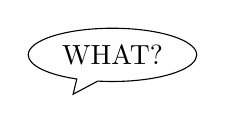
\begin{tikzpicture}
					\node[ellipse callout,draw, callout absolute pointer={(0.5,0)}]   at (1,0.5)
					{WHAT?};
				\end{tikzpicture}
			}
			\begin{block}{Honest Claim}
				\begin{itemize}
					\item Explicit construction of an \alert{Homotopy co-momentum Map}
					\item w.r.t. a pair Lie algebra - MultiSymplectic manifold \\
							relevant to hydrodynamics %~
				\end{itemize}
			\end{block}
		\end{column}
		\begin{column}[T]{0.5\textwidth} 
	        \centering
	        \resizebox {0.85\columnwidth} {!} {
				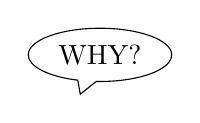
\begin{tikzpicture}
					\node[ellipse callout,draw, callout absolute pointer={(0.75,0)}]   at (1,0.5)					{WHY?};
				\end{tikzpicture}
			}
			\begin{block}{Honest Motivation}
				\begin{itemize}
					\item Provide an application of the Homotopy co-momentum Map machinery
						related to a mechanical problem
				\end{itemize}
			\end{block}		
		\end{column}
		%
		\note{
			\textbf{\underline{OUTLINE}}:
			\tableofcontents
		}
	\end{columns}
	\vspace{2ex}
	\begin{keywordblock}
		\begin{tabular}{|c|c|c|}
			\hline 
			symplectic & $\rightsquigarrow$ & multisymplectic \\ 
			\hline 
			Observables (Poisson) algebra & $\rightsquigarrow$ & Observables $L-\infty$ algebra \\ 
			\hline 
			Co-moment map & $\rightsquigarrow$ & Homotopy co-momentum map \\ 
			\hline 
		\end{tabular} 
	\end{keywordblock}
  \end{frame}
%---------------------------------------------------------------------------------------------------------------------------------------------------


%--------------------------------------------------------------------------------------------------------------------------------
\section{Background Material} 
\checkpoint
%--------------------------------------------------------------------------------------------------------------------------------
  \subsection{Multisymplectic manifolds}
  \begin{frame}[fragile]{Multisymplectic Manifold} %Fragile -->workaround tikzcd
			\begin{defblock}[$n$-plectic manifold]
				%
				\tikzstyle{every picture}+=[remember picture]
				\everymath{\displaystyle}
				\tikzstyle{na} = [baseline=-.5ex]
				%
				\begin{columns}
			    \begin{column}{.3\linewidth}
			    			\begin{displaymath}
							 (
							 \tikz[baseline]{
							            \node[fill=blue!20,anchor=base] (t1)
							            {$ M$};
							        } 
								,
								 \tikz[baseline]{
							            \node[fill=blue!20,anchor=base] (t2)
							            {$ \omega$};
								}
							)
						\end{displaymath}	
			    \end{column}
			    %
			    \begin{column}{.6\linewidth}		
					\begin{itemize}
					    \item[] \tikz[na] \node[coordinate,fill=blue!20,draw,circle] (n1) {};		    
					   		 Smooth Mfd.
					        
					    \item[] \tikz[na]\node [coordinate,fill=blue!20,draw,circle] (n2) {};	    
					    		(weakly) \alert{non-degenerate}, closed, $(n+1)$ form
			
					\end{itemize}
			    \end{column}
			    \end{columns}
				%
				\begin{tikzpicture}[overlay]
				        \path[->] (n1) edge [bend right] (t1);
				        \path[->] (n2) edge [bend left] (t2);
				\end{tikzpicture}
				%
			\end{defblock}

			\begin{defblock}[Non-degenerate n-form]
				\begin{columns}
					\hfill
					\begin{column}{.4\linewidth}
						\centering{
						The multi-contraction map $\alpha^{(j)}$\par
						is injective in the case $j=1$.
						}
					\end{column}
					\begin{column}{.6\linewidth}
						\[
						\begin{tikzcd}[column sep= small,row sep=0ex]
						    \alpha^{(j)} \colon& \mathfrak{X}^j(M) 	\arrow[r]& 				\Omega^{n+1-j}(M) \\
						  						& \xi_1\wedge\ldots\wedge\xi_j 						\arrow[r, mapsto]& 	\iota_{\xi_j}\cdots\iota_{\xi_1} \omega 					
						\end{tikzcd}	
						\]
					\end{column}
				\end{columns}
			\end{defblock}

			\begin{itemize}
					\item multisymplectic means \emph{going higher} in the degree of $\omega$
					\item 1-plectic $=$ symplectic
			\end{itemize}
			\vspace{1ex}
			\pause
			\begin{block}{Example:}
				Any oriented $(n+1)$-dimensional manifold is $n$-plectic w.r.t. the volume form.
			\end{block}			 


  \end{frame}
  \note[itemize]{
  	\item Notation: in the following, we will suppress $M$ when denoting the spaces of tangent fields $\mathfrak{X}(M)$ and differential forms $\Omega^n(M$)
  	\item Remark: introducing the notation of multi-contraction could seem an overkill at this point. However it will be useful in the following.
  	%Hiny by Ori
  	\item Weak is an $\infty$-dimensional condition on sections. Usually (for instance in the tautological form construction) is used a stronger condition:\\
		The bundle map $\alpha: TM \rightarrow \wedge^n M$, acting on fibers as
		$\alpha_x : v_x \to \iota_{v_x} \omega_x$
		is injective on every fibers.  
		\item the strong implies the weak: a bundle map between bundles on the same base induce a map between sections.
		\item The converse is not true. Consider $\omega = x \text{d}x \wedge \text{d}y$, a presymplectic form that is not degenerate only on a dense domain.
		The map induced on section is injective
		$$\Gamma(T\mathbb{R}^2) \rightarrow \Gamma(T^\ast\mathbb{R}^2) : f\partial_x + g\partial_y \to x \left(f \text{d}y - g \text{d} x\right)$$
		because the r.h.s. vanish only when $f,g$ are zero on $\mathbb{R}^2 \ \text{y-axis}$ but since $f,g$ are coefficient of smooth field, the continuity implies that such functions vanish everywhere.
		
		}
%---------------------------------------------------------------------------------------------------------------------------------------------------


%------------------------------------------------------------------------------------------------
  \begin{frame}[fragile]{A significant example} 
		Consider a smooth manifold $Y$,
		\begin{columns}
			\hfill
			\begin{column}{.5\linewidth}
				\emph{Multicotangent bundle} $\bigwedge = \bigwedge^n T^\ast Y$\\
				is naturally $(n+1)$plectic
			\end{column}
			\begin{column}{.4\linewidth}
				\[
				\begin{tikzcd}
					\Lambda \ar[d,"\pi"'] & T \Lambda \ar[d,"T \pi"] \ar[l] \\
					Y								& T Y \ar[l]
				\end{tikzcd}	
				\]
			\end{column}
		\end{columns}
	\vspace{2ex}
	\begin{defblock}[Tautological $n$-form]
		$\theta \in \Omega^n(\Lambda)$ such that:
		\begin{displaymath}
		\begin{split}
			\left[ \iota_{u_1 \wedge \ldots \wedge u_n} \theta \right]_\eta 
			&= \iota_{(T \pi)_\ast u_1 \wedge \ldots \wedge (T \pi)_\ast u_n} \eta \\
			&= \iota_{u_1 \wedge \ldots \wedge u_n} \pi^\ast \eta 
			\qquad \qquad \forall \eta \in \Lambda \, , \: \forall u_i \in T_\eta \Lambda 		
		\end{split}
		\end{displaymath}
	\end{defblock}
		\begin{columns}
			\begin{column}{.6\linewidth}
				\begin{defblock}[Tautological (multisymplectic) (n+1)-form]
					$$\omega := d \theta$$
				\end{defblock}
			\end{column}
			\begin{column}{.4\linewidth}
			 	\begin{claimblock}$\omega$ is not degenerate.\end{claimblock}	
			\end{column}
		\end{columns}	
		\vspace{2ex}
		\begin{itemize}
			\item \emph{Higher analogue} of the cotangent bundle.
			\item (but is not yet the analogue of a \emph{phase space}.)
		\end{itemize}
  \end{frame}
  		\note[itemize]{
  			\item This example is significant from the perspective of geometric classical field theory.
			\item Recall the notation of multi-contraction: $\iota_{u_1 \wedge \ldots \wedge u_k} = \iota_{u_k}\cdots\iota_{u_1}$;
			\item A sketch of the proof of non degeneracy could be found in the appendix, pag: \ref{frame:multicotangentismultisymp}.
			\vspace{1ex}
			\begin{columns}
					\begin{column}{.6\linewidth}
						Informally, the gist of the tautological form can be summarized as the unique way to get a number out any $\eta\in \wedge^n T^\ast M$ when you have at hands only tangent vectors on the bundle $\wedge^n T^\ast M$ \\
						More precisely, is the unique differential form on $\wedge^n T^\ast M$ which value in a point $\eta$ when contracted with tangent vector $v_1 \ldots v_k$ is equal to to the value of $\eta$ when contracted with the drop on $Y$ of the same vectors.
					\end{column}
					\begin{column}{.4\linewidth}
						\includestandalone[width=\textwidth]{Pictures/Figure_tautologicalform}
					\end{column}
			\end{columns}				 	
		}
%--------------------------------------------------------------------------------------------------------------------------------------------------- 
  
  
%------------------------------------------------------------------------------------------------
  \begin{frame}[fragile]{Geo-Mech. motivation for multisymplectic} 
	Consider a smooth bundle $\pi: E\rightarrow \Sigma$
	\vspace{1em}
  	\begin{defblock}[pre-multiphase space]
		\begin{columns}
		%
	    \begin{column}{.4\linewidth}
			\[
			\begin{tikzcd}[column sep= small,row sep=small]
				\Lambda^n_k  \ar[rr,hookrightarrow,"i"] \ar[dr]& & \bigwedge^n T^\ast E \ar[dl]\\
				& E \ar[d,"\; \pi"] & \\
				& \Sigma &
			\end{tikzcd}	
			\]
	    \end{column}  
		%
		    \begin{column}{.6\linewidth}
			    	\begin{displaymath}
				    	\begin{split}
				    		\big(\Lambda^n_{\, k} \big)_y = 
				    		\big\lbrace \eta \in \Lambda \, \big\vert \;& \iota_{u_{k+1}}\ldots \iota_{u_1} \eta = 0 \\
				    		& \forall u_i \in V_y(\pi) = ker(\pi_\ast)_y \big\rbrace
				    	\end{split}	    		
			    	\end{displaymath}
			    	Multisymplectic with $i^\ast \omega$.
		    \end{column}  
		%
		\end{columns}
  	\end{defblock}
  	
	\begin{table}[]
	\begin{tabular}{|p{14em}|p{14em}|}
		\hline
		\textbf{Mathematics}                   & \textbf{Physics}\\
		\hline
		Smooth bundle							  & Configuration Bundle \\
		K-plectic manifold                       & Multiphase space of a system with infinite degrees of freedom\\ 
		& \footnotesize ($k-1$ dimensional space of DOF)\\
		Submanifold of dimension k  (section if M is a bundle) & States as dynamical configuration  \\
		$L-\infty$ algebra of observables                     & Measurable quantities\\
		\hline
	\end{tabular}
	\end{table}
  \end{frame}
  \note[itemize]{
  	\item Recall: $V_y(\pi) = ker(\pi_\ast)_y$ are vertical vector fields.
  	\item The multiphase space is the sub-bundle of $n$-forms vanishing when contracted with $k$ vertical fields.
  	\item The table is a dictionary between the mathematical objects and their role in the geometric mechanics of  system with  a k-1 dimensional continuum of DOF.
  	\item Warning: (about the physical state) in classical mechanics is customary to confuse trajectories with initial data.
  	\item The reason why this sub-bundle has a particular role is that it can be proved to be isomorphic to a suitable dual of the first Jet bundle.
  	\item For further details see Gotay et al.\href{https://arxiv.org/abs/physics/9801019}{arXiv:physics/9801019}. For a pictorial representation of all the structures involved in the geometric mechanics of I order classical field theories see appendix, pag: \ref{frame:Gimmsy}.
  	
  }
%---------------------------------------------------------------------------------------------------------------------------------------------------


%------------------------------------------------------------------------------------------------
  \begin{frame}{Special classes of smooth objects} 
  	\begin{columns}
		\begin{column}[t]{.42\linewidth}		
			\begin{defblock}[Hamiltonian v.f.]
				$\mathfrak{X}_{ham} =  \left\lbrace X \in  \mathfrak{X} \right\vert \left. \iota_x \omega \textrm{ exact}  \right\rbrace$ 			
			\end{defblock}
			\begin{defblock}[Multisymplectic v.f.]
				$\mathfrak{X}_{ms} =  \left\lbrace X \in  \mathfrak{X} \right\vert \left. \mathcal{L}_X \omega = 0  \right\rbrace$ 	
			\end{defblock}
		\end{column}
		\begin{column}[t]{.58\linewidth}		
			\begin{defblock}[Hamiltonian $(n$-$1)$forms]
				$\Omega^{n-1}_{ham} =  \left\lbrace H \in  \Omega^{n-1} \right\vert \left.  \exists X \in \mathfrak{X}_{ham} \; : \;d H = \iota_x \omega \right\rbrace$ 			
			\end{defblock}		
		\end{column}
  	\end{columns}
  	%
  	\vspace{0.5em}
  	%
  	\onslide<2->{
  	\begin{columns}
		\begin{column}[t]{.5\linewidth}	
			\centering\emph{Global symmetries}
			\begin{defblock}[Multisymplectic (Lie group) action]
				$\Phi: G \circlearrowright (M, \omega)$ \emph{right action} s.t. \\
				$$\hat{\Phi}(g)_\ast \omega = \omega \quad \forall g \in G$$
			\end{defblock}
		\end{column}
		\begin{column}[t]{.5\linewidth}			
			\centering\emph{Infinitesimal symmetries}
			\begin{defblock}[Multisymplectic (Lie algebra) action]
				$V: \mathfrak{g} \rightarrow \mathfrak{X} (M)$ \emph{Lie algebra morphism} s.t. \\
				$$\mathcal{L}_{V_\xi} \omega = 0 \quad \forall \xi \in \mathfrak{g}$$	
			\end{defblock}
		\end{column}
  	\end{columns}
  	}
  	%
  	\onslide<3->{		
	  	\begin{asideblock}[Hierarchy of conserved quantities]%Shades of...
	  		\begin{table}[] % http://tablesgenerator.com/
			\begin{tabular}{lllll}
					& strictly conserved & & & $\mathcal{L}_X \alpha= 0$ \\
				$\alpha \in \Omega^\bullet$ & globally conserved & along $X \in \mathfrak{X}$ & $\Leftrightarrow$ & $\mathcal{L}_X \alpha\in B $ (exact) \\
				  & locally conserved  & & & $\mathcal{L}_X \alpha\in Z $ (closed)                                
			\end{tabular}
			\end{table}
	  	\end{asideblock}
  	}
  	
  \end{frame}
  \note[itemize]{
  	\item Exactly as it happens in symplectic geometry, fixing a smooth form $\omega$ on $M$ yields a criterion for classifying vector fields and differential forms.
  	\item Also, we can naturally select a special class of symmetries (global and infinitesimal) which preserve the fixed multisymplectic form.
  	\item Aside, we can start to see that, in this setting, measurable quantities are not only smooth functions but also differential forms with degree greater then zero.
  	For such objects can be defined weaker notions of conservation along a flow.
  	\item The idea to consider forms of various degree as observables do not fall out of the sky. 
  		For instance in a string there will be two kind of measurable quantities: extensive observable (1-forms), like the density, and intensive observables (0-forms), like the tension. 
 		%\href{https://en.wikipedia.org/wiki/Intensive_and_extensive_properties#Intensive_properties}{(wiki link on this terminology)}
  	\item Starting from this observation we can define the space of all possible observables (see next slide).
  }
%---------------------------------------------------------------------------------------------------------------------------------------------------


%---------------------------------------------------------------------------------------------------------------------------------------------------
  \subsection{Lie $\infty$-algebra of Observables}
  \begin{frame}[fragile,t]{Lie $\infty$-algebra of Observables \emph{(Rogers)}}
  	Consider $(M,\omega)$, $n$-plectic manifold,
	\begin{defblock}[$L-\infty$ Algebra of observables]
		Is a chain-complex\\
		\ifHandout
			\includestandalone[width=\textwidth]{Pictures/Figure_Observables}	
		\else
			\includestandalone[width=\textwidth]{Pictures/Frame_Observables}
		\fi
		\onslide<2->{with $n$ multibrackets $(2 \leq k \leq n+1)$\\
			\includestandalone[width=0.7\textwidth]{Pictures/Equation_Multibracket}
		}
		\only<2->{	\footnote{$\varsigma(k) := - (-1)^{\frac{k(k+1)}{2}}$}}

	\end{defblock}

%  \onslide<3->{
		\begin{itemize}
			\item \emph{higher analogue} of the \emph{Poisson algebra structure} associated to a symplectic manifold.
		\end{itemize}
	%}
  \end{frame}
 \note[itemize]{
	 \item What is a $L-\infty$ of observables?\\
		Basically, is a chunk of the de Rham complex of $M$ with inverted grading and an extra structure, namely the multibrackets.
 	\item Take away message: the "space of observables" on a ms. mfd. carry the structure of a $L-\infty$ algebra.\\
 		( In the symplectic case it reduces to the corresponding Poisson algebra)
 	\item Rogers associated to any n-plectic mfd a $L-\infty$ algebra.
 	\item Zambon generalized to it pre n-plectic.
 	\item Remark: recognize in the definition of $[\cdot,\ldots,\cdot]_k$ the contraction with hamiltonian fields.
 	\item This definition is a special instance of a more general object  called L$-\infty$ Algebra. \\
 		An $L-\infty$ algebra is a notion that one obtains from a Lie algebra 
 		requiring that the Jacobi identity is satisfied only up to a higher coherent chain homotopy.
 }
%------------------------------------------------------------------------------------------------


%------------------------------------------------------------------------------------------------
  \subsection{Homotopy co-momentum map}
  \begin{frame}[fragile,t]{Homotopy co-momentum map \emph{(Callies, Frégier, Rogers, Zambon)}}
  	%
		Consider a multisymplectic action $G \circlearrowright (M, \omega)$,
		%
		\begin{defblock}[Homotopy co-momentum map (HCMM)]				
			Is a sequence of linear maps:
			\begin{displaymath}
				(f)  = \big\lbrace f_k: \; \Lambda^k{\mathfrak g} \to L_{k-1} \subseteq \Omega^{n-k} 
				\;\big\vert\; 0\leq k \leq n+1  \big\rbrace
			\end{displaymath}
			%
			\includestandalone[width=0.95\textwidth]{Pictures/Frame_HCMM}			
			\emph{such that:}
			\begin{itemize}
				\item $f_0 = 0 $, $f_{n+1} = 0$ %(we have tacitly set $\Lambda^{-1}(M) = 0$)
				\item<2-> $-f_{k-1} (\partial p) = d f_k (p) + \varsigma(k) \alpha^{(k)} \quad \forall (k=1,\dots n+1), \; \forall p \in \Lambda^k(\mathfrak{g})$
			\end{itemize}
		\end{defblock}
		\begin{itemize}
			\item \emph{Higher analogue} of the ordinary co-moment map $f\colon \mathfrak{g}\rightarrow C^\infty(M)$.
		\end{itemize}
  \end{frame}
  \note[itemize]{
		\item Notice that a HCMM pertains to an "infinitesimal" action of ${\mathfrak g}$ on $M$ 
			with ${\mathfrak g}$ being the Lie algebra of a generic Lie group $G$, 
			acting on $M$ by $\omega$-preserving vector fields.
		\item (Notation) $ p = \xi_1 \wedge \xi_2 \wedge \dots \wedge \xi_k$, 
			then $v_p = v_1 \wedge v_2 \wedge \dots \wedge v_k$ 
			where $v_i \equiv v_{\xi_i}$ are the fundamental vector fields associated to the action of $G$ on $M$
	%	\item (Notation) $\iota(v_p) \omega = \iota(v_k)\dots\iota(v_1) \omega$
	%	\item $\varsigma(k) := - (-1)^{\frac{k(k+1)}{2}}$ 
		\item (Recall) $\alpha^{(k)}\coloneqq \iota(v_p) \omega = \iota(v_k)\dots\iota(v_1) \omega$
		\item $\partial \equiv \partial_k:  \Lambda^{k} {\mathfrak g} \to \Lambda^{k-1} {\mathfrak g}$  is the usual Eilenberg-Chevalley complex boundary operator (see appendix, pag: \ref{frame:CE-complex});
		\item The definition tells us that the {\it closed} forms
			$$\mu_k := f_{k-1} (\partial p) +  \varsigma(k) \iota(v_p) \omega 	$$
			must actually be {\it exact}, with potential $-f_k(p)$.  	
		\item The last equation tells us that an HCMM is not a chain complex morphism but is rather a chain complex homotopy between 0 and the multicontraction $\alpha$ (is a chain map by lemma 2.18 \cite{Ryvkin2016}).
		\item More concisely, an HCMM is a L-$\infty$ morphism $(f):\mathfrak(g)\rightarrow L(M)$.
  }
%------------------------------------------------------------------------------------------------


%------------------------------------------------------------------------------------------------
\section{An application in hydrodynamics}
\checkpoint
%------------------------------------------------------------------------------------------------


%---------------------------------------------------------------------------------------------------------------------------------------------------
  \begin{frame}{Hydrodynamical $\mathfrak{g}$- action}
	\begin{columns}[T] % align columns
	\begin{column}{.4\textwidth}
			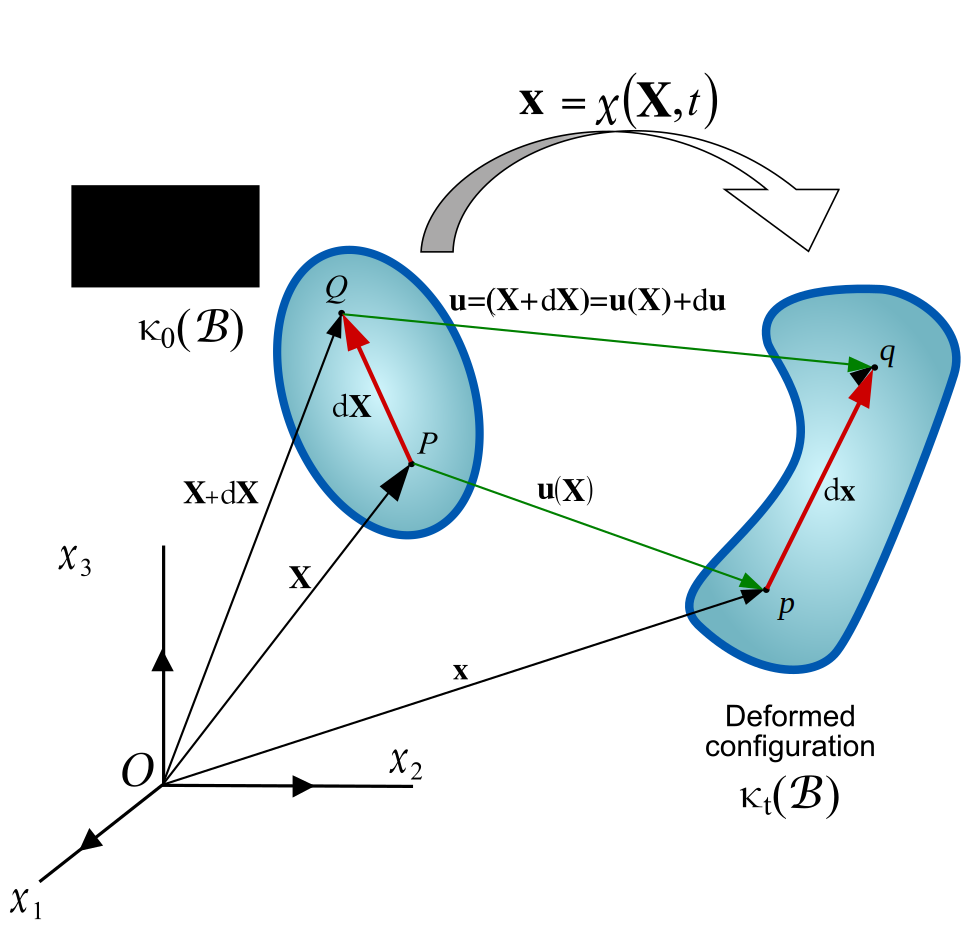
\includegraphics[width=\linewidth]{Pictures/Continuum_body_deformation}
	\end{column}
	%
	\hfill
	%
	\begin{column}{.6\textwidth}
		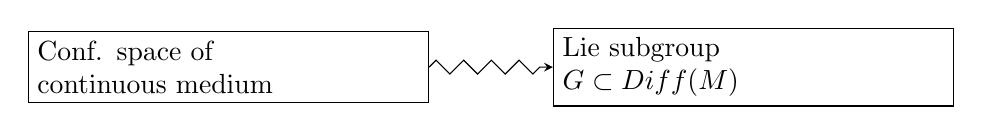
\begin{tikzpicture}[
			text width=0.4\linewidth,
			node distance=0.55\linewidth,
			]
			\node [rectangle,draw] (lhs) {Conf. space of\\ continuous medium};
			\node [rectangle,draw,right of=lhs] (rhs) {Lie subgroup \\$G \subset Diff(M)$};
			\path [snake=zigzag,-stealth,draw] (lhs) -- (rhs);
		\end{tikzpicture}

		Examples:
		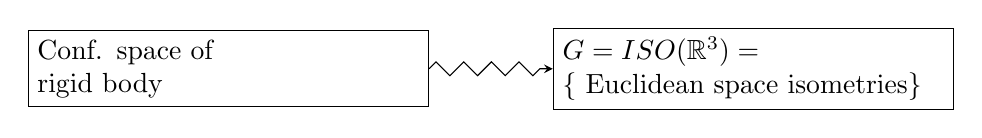
\begin{tikzpicture}[
			text width=0.4\linewidth,
			node distance=0.55\linewidth,
			]
			\node [rectangle,draw] (lhs) {Conf. space of\\ rigid body};
			\node [rectangle,draw,right of=lhs] (rhs) {$G=ISO(\mathbb{R}^3)=$\\ $\{$
				Euclidean space isometries$\}$};
			\path [snake=zigzag,-stealth,draw] (lhs) -- (rhs);
		\end{tikzpicture}
		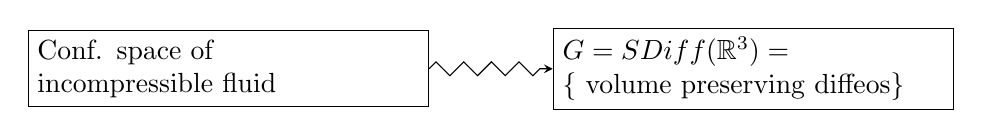
\begin{tikzpicture}[
			text width=0.4\linewidth,
			node distance=0.55\linewidth,
			]
			\node [rectangle,draw] (lhs) {Conf. space of\\ incompressible fluid};
			\node [rectangle,draw,right of=lhs] (rhs) {$G= SDiff(\mathbb{R}^3)=$\\ $\{$
				volume preserving diffeos$\}$};
			\path [snake=zigzag,-stealth,draw] (lhs) -- (rhs);
		\end{tikzpicture}
	\end{column}%
	\end{columns}
		%
  	\begin{propblock}[$(\mathbb{R}^3,\nu = dx\wedge dy\wedge dz)$ is 2-plectic]
  		\begin{itemize}
  			\item \emph{(Easy proof)} $\quad \iota_v \nu = \frac{1}{2}\epsilon_{i j k} v^i dx^j \wedge dx^k = 0 \; \Leftrightarrow \; v=0 $;
  			\item \emph{(Conceptual proof)} $\quad \alpha^{(1)} = \ast \circ \flat$ is invertible.
  		\end{itemize}
  	\end{propblock}
%		\begin{claimblock} Any oriented manifold is multisymplectic w.r.t. the volume form. \end{claimblock}

		\onslide<2->{
		 	Consider a subalgebra of the infinitesimal action of $SDiff(\mathbb{R}^3)$:
		  	\begin{displaymath}
		  		\mathfrak{g} = sdiff_0(M) = \lbrace  X \in \mathfrak{X} \quad\vert\quad div X = 0, \textrm{\emph{ rapidly vanishing at }}\infty \rbrace
		  	\end{displaymath}
		  	\centering \alert{(Infinite dimensional Lie algebra!)}
	  	}
  
  \end{frame}
  \note[itemize]{
	%\item  Now we are ready to get to the real business. Namely, give an explicitly construction of a HCMM related to hydrodynamics.
	\item We are working in the setting of \emph{geometric continuum mechanics} .\\
		Recall that the configuration space of a continuum object is encoded via diffeomorphisms. In the case of an incompressible fluid is encoded via volume-preserving diffeomorphisms.
	\item Such manifold are infinite dimensional. Particular caution has to be taken when defying in what sense such manifold is smooth.
	\item However, what really pertains to the construction of a moment map is the infinitesimal action, i.e. the Lie algebra. In our case, the infinitesimal action to be considered is via divergence-free vector fields.
	\item (Notation): In the following M will be the 3 dimensional Euclidean Space.
	\item The key, but trivial, observation is that the standard volume form on the euclidean space is a multisymplectic form.
	\item In the following, we will see that the standard Riemannian structure takes a role in our construction. 
	That the reason to show also a "conceptual proof".
	\item Notation: $\ast = $ and $\sharp = $ are respectively the Hodge operator and the Riemmanian sharp operator pertaining to the standard metric in $\mathbb{R}^3$.	
  }
%------------------------------------------------------------------------------------------------


%------------------------------------------------------------------------------------------------
  \subsection{Explicit Construction of the HCMM}
  \begin{frame}{Hydrodynamical homotopy co-momentum map}
  	\begin{claimblock}
  		Explicit construction of an HCMM for $SDiff_0 \circlearrowright (\mathbb{R}^3,\nu)$
  	\end{claimblock}
	\begin{columns}
		\begin{column}[c]{.5\linewidth}
		  	\begin{itemize}
		  		\item The observables are  $$L= \Omega^1_{\textrm{ham}}(\mathbb{R}^3)\oplus\Omega^0(\mathbb{R}^3)$$
		  		\item HCMM consists of a pair of functions:
					\begin{align*}
						f_1 &\colon \mathfrak{g} \rightarrow \Omega^1_{\textrm{ham}}(\mathbb{R}^3) \\
						f_2 &\colon \mathfrak{g}\wedge\mathfrak{g} \rightarrow C^\infty(\mathbb{R}^3)
					\end{align*}	
		  	\end{itemize}
		\end{column}	
	  	\hfill  	
		\begin{column}[c]{.5\linewidth}
  		\includestandalone[width=\textwidth]{Pictures/Figure_Euclid_Trigger}
 	 	\end{column}
 	 \end{columns}
 	\begin{columns}
		\begin{column}[c]{.8\linewidth}
		 	 \begin{itemize}
				\item Satisfying the following system:
					\begin{displaymath}
						\begin{cases}
							\textrm{d} f_1(\xi) = \iota_\xi \nu = -\alpha^1(\xi) \\
							\textrm{d} f_2(\xi_1 \wedge \xi_2) = f_1\left([\xi_1,\xi_2]\right) - \iota_{\xi_2}\iota_{\xi_1} \nu 
							 \coloneqq \mu_2(\xi_1,\xi_2)\\
							f_2\left(\partial \xi_1 \wedge \xi_2 \wedge \xi_3 \right) = \iota_{\xi_3}\iota_{\xi_2}\iota_{\xi_1} \nu
						\end{cases}
					\end{displaymath}
		 	 \end{itemize}
 	 	\end{column}
		\begin{column}[c]{.2\linewidth}
 	 	\end{column}
 	 \end{columns}
  \end{frame}
	\note[itemize]{
		\item (Regarding the diagram)
		\item On the left there is the part of the Chevalley-Eilemberg complex that interact with the L-$\infty$ algebra of observables.
		\item On the right there is the whole de Rham complex of the manifold $M=\mathbb{R}^3$.
		\item Even if only $\Omega^1$ and $\Omega^0$ take part in the definition of a $HCMM$, the Riemmanian structure determine a correspondence with the rest of the de Rham complex.
		\item In order to give an HCMM for this action is necessary to give a solution of the system of 3 equations below.
	}  
%---------------------------------------------------------------------------------------------------------------------------------------------------


%--------------------------------------------------------------------------------------------------------------------------------------------------- 
  \begin{frame}[t]{Explicit Construction of the HCMM}
  	\begin{columns}
			\begin{column}[]{.5\linewidth}
 		 	\end{column}
			\begin{column}[]{.5\linewidth}
 		 	\end{column}
 	 \end{columns}

		\begin{enumerate}
			\item<1-> Fix $\vec{b} \in \mathfrak{g}$ and define $f_1(b) \coloneqq -\vec{A}^\flat$.\\ 
				The first equation is equivalent to solve
				\begin{displaymath}
					\tag{equation of magnetostatic}
					{\rm curl}(\vec{A})=\vec{b}
				\end{displaymath}
				This equation admits a solution 
				\begin{displaymath}
					\tag{Biot-Savart law}
					\vec{A}(r) = \int\frac{\vec{b}\times(\vec{r}-\vec{r}')}{|\vec{r}-\vec{r}'|^3}\textrm{d}r'
				\end{displaymath}							
				\alert {Defined up to a gradient \emph{(gauge freedom)}}. 
			%
			\item<2-> $\mu_2(\xi_1,\xi_2)$ is closed $\forall \xi\in\mathfrak{g}$ $\xRightarrow[\text{lemma}]{\text{Poincar\'e}}$ is exact.\\
				%Hence it is also exact \emph{(Poincar\'e lemma)}.\\
				Take as $f_2(\xi_1,\xi_2)$ a primitive $0$-form, \alert{determined up to a constant $c(\xi_1,\xi_2)$}.
			%
			\item<3-> Third equation is a priori only true up to a constant $c(\xi_1, \xi_2, \xi_3)$.\\
				The constant is zero since $\nu(\xi_1, \xi_2, \xi_3)$ vanishes at infinity and 
				the same is true for $f_2(\partial q)$ upon solving the related Poisson equation
 				\begin{displaymath}
 			 		\Delta f_2(\partial q) = \Delta \nu(\xi_1, \xi_2, \xi_3)			
 				\end{displaymath}
		\end{enumerate}
  \end{frame}
  \note[enumerate]{
  	\item	
  		\begin{itemize}
		  	\item Exploiting the correspondence between tangent fields and 1-form given by the metric is possible to recast the first equation in a simple vector calculus equation containing  the curl.
		  	\item Such equation is the well-known equation of magnetostatic with admits solution by the Biot-Savart law.
		  	\item In the context of hydrodynamic $A$ can be interpreted as a \emph{velocity field} and $b$ as the corresponding vorticity. (See slide for further details)  		
  		\end{itemize}
  	\item In the language of physics, such primitive form is often called "a potential".
  	\item 
  		\begin{itemize}
  			\item (Notation) $q = \xi_1 \wedge \xi_2 \wedge x_3$.
  			\item Last equation tells us that $f_2(\partial q)$ and $ \nu(q)$ differs by a constant. But since both of them vanish at infinity this constant has to be zero.
  			\item The condition of vanishing at infinity has been imposed in order to fulfil the last equation.
  		\end{itemize}
  	\item[$\triangleright$] This construction can be generalized to oriented Riemannian manifolds with further cohomological condition. 
  		See appendix, pag: \ref{frame:RiemannianGeneralization}.
  }
%---------------------------------------------------------------------------------------------------------------------------------------------------


%---------------------------------------------------------------------------------------------------------------------------------------------------
  \subsection{Hydrodynamics interpretation}
  \begin{frame}[fragile]{Hydrodynamics interpretation}
		Consider the loop spaces $L{\mathbb R}^3$,\\
		%
		\begin{propblock}[HCMM for $G\circlearrowright(\mathbb{R}^3,\nu)$ induces \\an ordinary co-mo.map for $G\circlearrowright (LS,\nu^{\ell})$]
			The HCMM $f \colon \mathfrak{g} \to L_{\infty}(\mathbb{R}^3,\nu)$ previously given
			\emph{transgresses}	 to
			\begin{displaymath}%\tag{Arnol'd-Marsden-Weinstein\\ hydrodynamical co-momentum map}
				\begin{tikzcd}[column sep= small,row sep=0ex]
					\lambda \colon& \mathfrak{g}	\arrow[r]& C^\infty(LS) \\
					& {\mathbf b}	\arrow[r, mapsto]& \displaystyle \lambda_b(\textvisiblespace) =-\oint_{\textvisiblespace} B^\beta = - \oint_{\textvisiblespace} f_1({\mathbf b}) 
					%	\quad \forall \gamma \in LS		
				\end{tikzcd}	
			\end{displaymath}
			that is a  moment map for the induced action $G$ on the pre-symplectic loop space $(LM,\nu^{\ell})$. (Smooth space in the sense of Brylinski)
		\end{propblock}
		\begin{itemize}
			\item $\lambda$ corresponds to \emph{Arnol'd-Marsden-Weinstein hydrodynamical co-momentum map}  defined on $\infty$-dim. manifolds.
			\item<2-> $\Lambda = \left\lbrace \lambda_{\mathbf b} \right\rbrace_{{\mathbf b}\in\mathfrak{g}}$ is, up to sign, the {\it Rasetti-Regge current algebra}
			\item<3-> There is a naturally defined a {\it Poisson brackets} on $\Lambda$:
				\begin{displaymath}
					\{ f_1({\mathbf b}), f_1({\mathbf c}) \} (\cdot):= \iota_{\mathbf c} \iota_{\mathbf b} \nu (\cdot)=
						\nu({\mathbf b}, {\mathbf c}, \cdot) = f_1([{\mathbf b},{\mathbf c}])
					-df_2 ({\mathbf b} \wedge {\mathbf c})
				\end{displaymath}
				\centering\footnotesize(Note: $\lambda$ is (infinitesimally) $G$-equivariant, i.e. $	\{\lambda_{\mathbf b}, \lambda_{\mathbf c} \} = \lambda_{[{\mathbf b}, {\mathbf c}]}$)
		\end{itemize}

    
  \end{frame}
  \note[itemize]{
  	\item[ ] \textbf{How all of this is relevant in Hydrodynamics?}
  	\item The loop space is the manifold, in the sense of Brylinsky, consisting of all smooth loops in ${\mathbb R}^3$.
  	\item Transgression can be seen as a pull-back along the evaluation map 
  		$${\rm ev}: L{\mathbb R}^3 \times {\mathbb R} \ni (\gamma, t) \mapsto \gamma(t) \in {\mathbb R}^3$$
  		  	For further details see appendix, pag: \ref{frame:LoopSpacesTransgression}.
  	\item Note that the (RR) current pertaining to ${\mathbf b} \in {\mathfrak g}$  is independent of the choice of $B$.
  			See appendix, pag: \ref{frame:RRcurrents} for other informations on this concept or \cite{Rasetti1975},\cite{Penna1992} for a deeper account.
  	\item In \cite{Callies2016} is proved a general result asserting that, roughly speaking,
			homotopy co-momentum maps transgress to homotopy co-momentum maps on loop (and even mapping) spaces. Further details in appendix, pag: \ref{frame:TransgressionHCMM}.
	\item Actually, the ansatz for $f_1$ term in the previous construction has been precisely motivated by this phenomenon. 
  }
 %------------------------------------------------------------------------------------------------

%------------------------------------------------------------------------------------------------
  \subsection{A connection with knot theory}
	\begin{frame}{A connection with Knot theory}
 		\centering$\Rightarrow$\emph{The bridge is the \alert{Vortex Dynamics}}$\Leftarrow$

		\begin{columns}
			\begin{column}[T]{.55\linewidth}
			 		\vspace{1ex}
 				$\bullet$Consider a perfect (incompressible, inviscid) fluid pervading the  whole space $M=\mathbb{R}^3$.\\
 				Its physical state is encoded by $u \in sdiff_0(\mathbb{R}^3)$
 				\begin{columns}
 					\begin{column}{.5\linewidth}	
 						\begin{defblock}[Vorticity]
							$\displaystyle \omega \coloneqq \textrm{curl}(u)$					
 						\end{defblock}
 					\end{column}
  					\begin{column}{.5\linewidth}	
 						\begin{defblock}[Helicity]
							$\displaystyle h = \int_{\mathbb{R}^3} u \cdot \omega  d^3x$		
 						\end{defblock} 		
 					\end{column}
 				\end{columns}
 				%
  				\begin{columns}
 					\begin{column}{.5\linewidth}	
						Dynamics is ruled by the \emph{Euler equation}:
						\begin{displaymath}
							\frac{\partial \omega}{\partial t} = [\omega, u]				
						\end{displaymath}
 					\end{column}
  					\begin{column}{.5\linewidth}	
						\begin{propblock}[Helicity is conserved]
							$\frac{d}{dt}H = 0$
						\end{propblock}
 					\end{column}
 				\end{columns}
 				\onslide<2->{
 					\vspace{2ex}
 					$\bullet$
	 				Consider now the case of $\omega$ localized in a flux loop $\mathcal{L}$.
	 				\begin{propblock}[Vortex filaments are preserved]
	 					$supp(\omega(0))\simeq supp(\omega(t)) \qquad \forall t$
	  				\end{propblock}
  				}
			\end{column}
			\begin{column}[T]{.40\linewidth}
				\vspace{-1ex}
				\begin{figure}[T]
						\onslide<3->{\caption{Knotted vortex in water  (Klenecker \& Irvine \cite{Kleckner2013})}}
						\onslide<2->{
							\href{https://www.nature.com/articles/nphys2560}{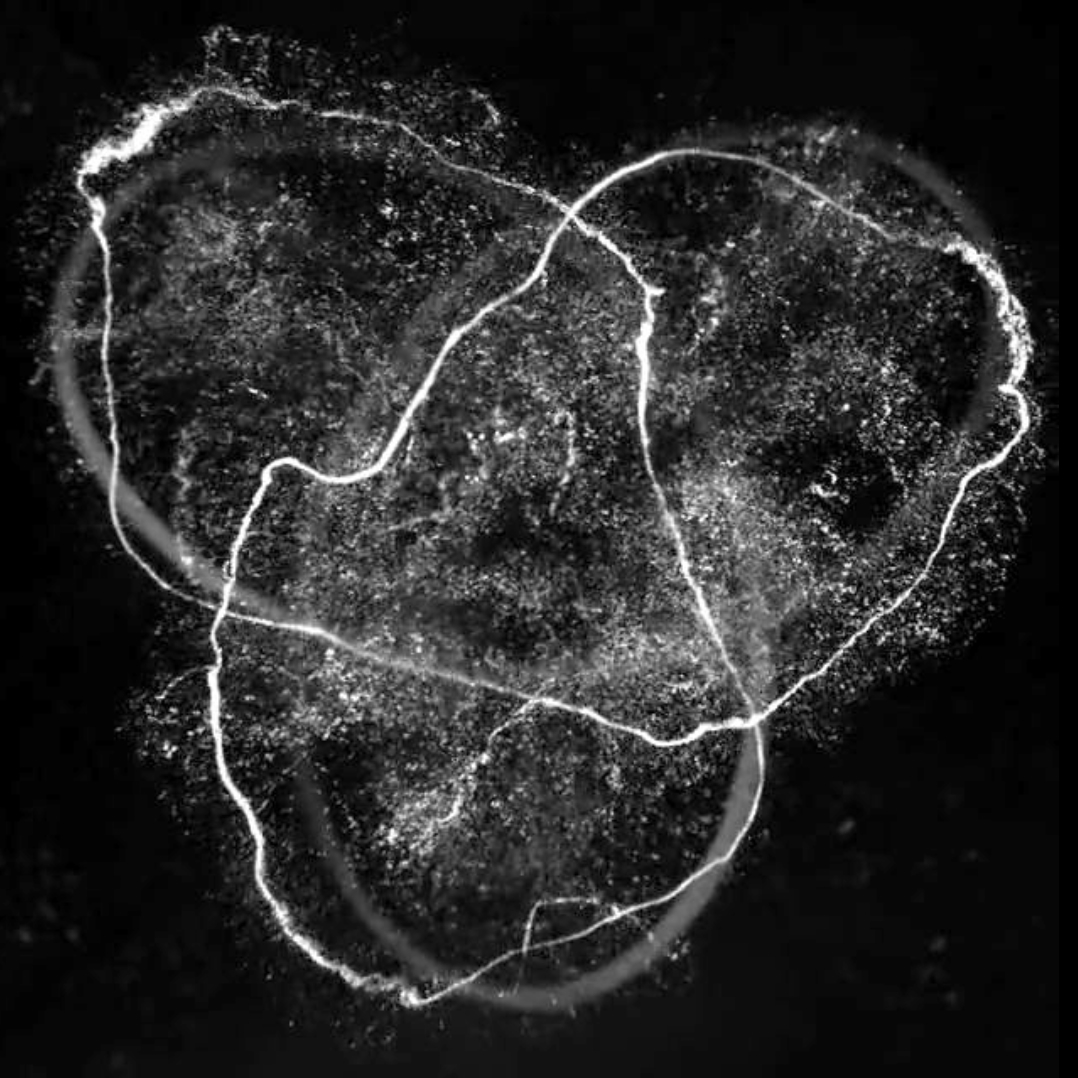
\includegraphics[width=\linewidth]{Pictures/knottedwatervortex}}		}
				\end{figure}
					\onslide<3->{
						\vspace{-2ex}
						\alert{Such fluid configurations are proved to exists both 
						\underline{theoretically} and \underline{experimentally}!}
					}
			\end{column}
		\end{columns} 
 \end{frame}
 \note[itemize]{
 	\item To find an application of this construction in knots theory is the main goal of our paper \cite{Miti2018}.
 	\item The first step is to notice that to any knot configuration can be associated a conserved form.
 }
%------------------------------------------------------------------------------------------------

%------------------------------------------------------------------------------------------------
  \begin{frame}{Conclusion}
		\begin{columns}
			\begin{column}{.45\linewidth}
				\onslide<2->{
				\begin{upshotblock}
					\begin{align*}
						f_1 &= \flat \circ {\rm curl}^{-1} \\
						f_2 &= {\rm grad}^{-1} \circ \sharp \circ \mu_2  
					\end{align*}						
					is a HCMM pertaining to the infinitesimal action of \\$\mathfrak{g}=sdiff_0$ on $\mathbb{R}^3$.
				\end{upshotblock}
				}
  	  \end{column}
			\begin{column}{.55\linewidth}
				\begin{itemize}
					\item We showed how to deal with observables and symmetries in multi-symplectic geometry;
					\item<2-> We described a natural example motivated by physics;\\
						\alert{$\Leftarrow$ momenta are related to vortices $\Leftarrow$}
					\item<3-> Transgression to loop spaces yields something already known in the context of fluid dynamics;		
				\end{itemize}
			\end{column}
			%	\hfill
    \end{columns}
    \vfill
    \begin{columns}
		\begin{column}{.60\linewidth} 
			\onslide<4->{
				\begin{block}{This exemplify a general phenomenon:}
					multisymplectic manifolds appear to be a \alert{"finite dimensional"} object able to encode features of \alert{"infinite dimensional"} mechanical systems.
				\end{block}
			}
		 \end{column}
		\begin{column}{.40\linewidth}   
			
			\ifHandout
					
			\else
				\centering
				\only<5->{\includestandalone[width=\textwidth]{Pictures/Animation_thankyou}}
			\fi
		 \end{column}		 
	 \end{columns}
  \end{frame}
  \note[itemize]{
		\item About the Upshot:
				\begin{itemize}
					\item Be aware of the sloppy notation: 
						the inverse of vector calculus differential operators are to be thought as their green operators.\\ 
						There is no unique inverse of the curl!
					\item Also the second one, is the operation of taking a primitive $f_2={\rm d}^{-1} \circ \mu_2 $.
				\end{itemize}
			\item We showed a natural example that is motivated by physics.\\
					This example uses an infinite dimensional group 
				(not all of the volume preserving diffeomorphisms but a big part of it.)\\
					This is also nice because the passing to loop spaces is natural and yields 
					something already known in the context of fluid dynamics.					
	}
%------------------------------------------------------------------------------------------------
  
%%%%%%%%%%%%%%%%%%%%%%%%%%%%%%%%%%%%%%
% APPENDIX
%%%%%%%%%%%%%%%%%%%%%%%%%%%%%%%%%%%%%%
\appendix
\section{EXTRA}
%\sectionpage
\begin{frame}
	\begin{center}
	\Huge\emph{EXTRA}
	\end{center}
\end{frame}
\addtocounter{framenumber}{-1}

%------------------------------------------------------------------------------------------------
 \begin{frame}[fragile,shrink]{Multicotangent bundle is multisymplectic} \label{frame:multicotangentismultisymp}
 	\begin{propblock}[$\omega$ is not degenerate. (Prop. 2.14 \cite{Ryvkin2018})]
		Non-degeneracy means that
		$$ \iota_{v_0} \omega = 0 \Leftrightarrow v_0 = 0 $$
		Consider coordinate chart $(U; y_i)$ on Y and induced coord. $(V; y_i, p_I)$ on $\Lambda$ 
		(with $I=(i_1,\ldots,i_n)$ strictly ascendent multi-index)\\
		W.r.t. such coordinates (Einstein's summation understood on $I$)
		$$ \theta = p_I\, dy^I \qquad \qquad \omega = -d p_I \wedge d y^I$$
		Therefore, take
		$$v_0 = a_i \dfrac{\partial}{\partial y^i} + b_I \dfrac{\partial}{\partial p_I}$$ 
		if $\exists J : b_J \neq 0 \quad \Rightarrow \iota_{v_0} \omega = b_J dy^J + \ldots$ \\
		if $b_I = 0 \forall I, \quad a_i \neq 0 (wlog\, i=1)$ consider $v_1= \dfrac{\partial}{\partial p_{(1,\ldots,n)}}$ and $v_j=\dfrac{\partial}{\partial y_j} \quad j>0$
		we have
		$$\iota_{v_0\wedge v_1 \wedge \ldots v_n} \omega = -a_1 \neq 0 $$
	\end{propblock}
 \end{frame}  
 %------------------------------------------------------------------------------------------------

 %------------------------------------------------------------------------------------------------
  \begin{frame}[fragile,t]{Chevalley-Eilenberg Complex}\label{frame:CE-complex}
  	Consider $\mathfrak{g}$, Lie Algebra.
  	\begin{defblock}[Eilenberg-Chevalley Complex]
  		Chain Complex
			\begin{center}
				\begin{tikzcd}[column sep= small,row sep=0.25ex]
					\ldots \ar[r,"\partial"] & \wedge^k \mathfrak{g} \ar[r,"\partial"] & 
					\wedge^{k-1} \mathfrak{g} \ar[r,"\partial"] & \ldots
			\end{tikzcd}	
			\end{center}
			with chain group
			\begin{displaymath}
				C^k := \wedge^k \mathfrak{g} \equiv 
				\big\{ c : \mathfrak{g}^\ast\times\ldots\mathfrak{g}^\ast \to \mathbb{R}\:\big\vert\, \textrm{alternating, k-linear} \big\}
			\end{displaymath}
			and boundary operator defined as
			$\partial \equiv \partial^k :  \Lambda^{k} {\mathfrak g} \to \Lambda^{k-1} {\mathfrak g}$  via
			$$
				\partial (\xi_1 \wedge \xi_2 \wedge \dots \wedge \xi_k) := \sum_{1\leq i< j \leq k} (-1)^{i+j}\, [\xi_i, \xi_j] \wedge \xi_1 \wedge \dots {\hat \xi}_i \wedge \dots \wedge {\hat \xi}_j \wedge \dots \xi_k
			$$
			where $\hat{}$ denoting deletion and with $\partial_0 = 0$.
  	\end{defblock}
		\begin{claimblock}
			$$\partial^2 = 0$$
		\end{claimblock}		
  \end{frame}
%------------------------------------------------------------------------------------------------

%------------------------------------------------------------------------------------------------
  \begin{frame}[shrink]{Riemannian Generalization}\label{frame:RiemannianGeneralization}
			\begin{columns}
				\begin{column}{.5\linewidth}
					\begin{itemize}
						\item  $(M,g)$ be a connected compact oriented Riemannian manifold of dimension $n+1$
						\item such that the {\it de Rham} cohomology groups $H_{dR}^{k}(M)$ vanish for $k=1,2,\dots n-1$ 
						\item endow it with the multisymplectic form $\nu$ given by its Riemannian volume form
						\item consider $g_0$, lie algebra consisting of divergence-free vector fields vanishing at a point $x_0 \in M$.
					\end{itemize}
					\begin{claimblock}
						$\exists (f)$, family of HCMM, pertaining to the infinitesimal action of $\mathfrak{g}_0$ on $M$
					\end{claimblock}
				\end{column}
				\begin{column}{.5\linewidth}
 			 		\includestandalone[width=\textwidth]{Pictures/Figure_Riemann_Trigger}
				\end{column}
			\end{columns}
		\textit{Sketch of proof:}\\
			The defining formula triggers a recursive construction starting from $f_1$.\\
			Take $ f_1(\xi) := -\Delta^{-1} \delta (\iota_{\xi} \nu)$
			$\quad$ (...) (see \cite{Miti2018})
  \end{frame}
  		\note[itemize]{
			%\item[(Thm)] A hydrodynamically flavoured HCMM can be similarly construed also for an $(n+1)$-dimensional connected, compact, orientable Riemannian manifold $(M,g)$, upon taking its Riemannian volume form $\nu$ as a multisymplectic form and again the group $G$ of volume preserving diffeomorphism group as symmetry group.
			\item[(recall)] The divergence of a vector field $X$ is defined via ${\rm div}\, X := *d\!*\!X^{\flat} = -\delta X^{\flat} $.
			\item The recursive construction start from $f_1$, up to topological obstructions  since we have a sequence of closed forms, which must be actually exact, together with the constraint $ f_n(\partial q) = (-1)^{\frac{(n+1)(n+2)}{2}}\nu(\xi_1,\dots\xi_{n+1})$, with $q= \xi_1 \wedge \dots \xi_{n+1}$, for the {\it constant} function $\mu_{n+1}(\cdot)$.
				\item A natural candidate for the (n-1)-form $f_1$ can be manufactured via Hodge theory as 
				$f_1(\xi) := -\Delta^{-1} \delta (\iota_{\xi} \nu)$
			after imposing $\delta f_1({\xi}) = 0$ (the analogue of the Coulomb gauge condition).
			\item Condition $H_{dR}^{n-1}(M) = 0$ assure one can safely invert the Hodge Laplacian $\Delta = d\delta + \delta d$;
			\item The 	topological assumptions made ensure that the entire procedure goes through unimpeded due to the formula
			$$
			df_k (\xi_1 \wedge\dots \wedge \xi_k) = \mu_k (\xi_1 \wedge\dots \wedge \xi_k), \qquad \qquad k=2,3,\dots n
			$$
			\item Finally, one has to check that 
			$$
			f_n (\partial (\xi_1 \wedge\dots \wedge \xi_{n+1})) =  -\varsigma(n+1) \iota (\xi_1 \wedge\dots \wedge \xi_{n+1})\nu
			$$
			this is guaranteed by the vanishing of all fields at $x_0$.
			% this is true once we notice that, since $c_{x_0} = 0$, the class $[c_x] = 0$ ( see \cite{Callies2016}, section 9).\qed
		}
%------------------------------------------------------------------------------------------------  

%------------------------------------------------------------------------------------------------
  \begin{frame}[fragile]{Loop spaces and transgression}\label{frame:LoopSpacesTransgression}
		\begin{columns}
			%
			\begin{column}[T]{0.5\textwidth}
				Consider any manifold $M$
				\begin{defblock}[Free loop space $LM$(Brilinsky)]
					$$ LM = C^\infty(S^{1},M)	$$
				\end{defblock}
			\end{column}
			%
			\begin{column}[T]{0.5\textwidth}		
				\begin{propblock}[$LM$ is an $\infty$-dimensional Fr\'echet manifold]		
					See \cite{Brylinski1993}.
				\end{propblock}
			\end{column}
			%
		\end{columns}
		
		\begin{defblock}[Tangent space at $\gamma \in LM$]
			\begin{displaymath}
				T_{\gamma}LM = C^\infty(S^{1},\gamma^{\ast}TM)= \Gamma^\infty(\gamma^\ast TM)	
			\end{displaymath}
		\end{defblock}

		\begin{defblock}[Trasgression]
			\begin{columns}
				%
				\begin{column}[t]{0.35\textwidth}
					\centering
					Degree $-1$ chain map
				\end{column}
				%
				\begin{column}{0.65\textwidth}
					\[
						\begin{tikzcd}[column sep= small,row sep=0ex]
					    \ell \colon& \Omega^{\bullet}(M) 	\arrow[r]& \Omega^{\bullet -1}(LM) \\
			  		  & \alpha (-)\arrow[r, mapsto]& 	\left.\alpha^{\ell} \right\vert_{\gamma} =
			    		\left.{\displaystyle\int^{2\pi}_{0} \iota_{\dot{\gamma}}\alpha(-)} \right\vert_{\gamma(s)} ~ ds
						\end{tikzcd}	
					\]
				\end{column}
				%
			\end{columns}
		\end{defblock}

		\begin{propblock}[Any pre-$n$-plectic structure $\omega$ on $M$ gives a pre-$(n-1)$-plectic structure $\omega^{\ell}$ on $LM$]
		Transgression commutes with the de Rham differential.
		\end{propblock}

		\note{
			\textbf{Intro by\cite{Callies2016}}\\
			\begin{displayquote}
			Homotopy moment maps for $G$-actions on pre-$2$-plectic manifolds $(M,\omega)$ can be transgressed to ordinary moment maps on the associated pre-symplectic loop space $LM$.

			Motivation for studying such actions arises, for example, in topological field theory. There one can consider a group of symmetries $G$ acting on a ``target space'' $M$ equipped with a closed form $\omega$.\\
The form can be transgressed to a mapping space $\mathrm{Map}(X,M)$ i.e.\ the ``space of fields''.\\ 

			Roughly speaking, this demonstrates how the higher symplectic geometry on $M$ can interact with the ordinary geometry on $\mathrm{Map}(X,M)$.		
			\end{displayquote}
		}    
  \end{frame}
%------------------------------------------------------------------------------------------------  

%------------------------------------------------------------------------------------------------
  \begin{frame}[fragile]{Transgression and HCMM}\label{frame:TransgressionHCMM}
  	\begin{propblock}[$G$-action on $M$ induces action on $LM$]
  		Given $G$-action $G \times M \to M$, we define a ``point-wise''  action $G \times LM \to LM$ given by:
		\[
			(g \cdot \gamma)(s) = g \cdot\gamma(s) \quad \forall g \in G, ~
			\forall \gamma \in LM
		\]
  	\end{propblock}
		
	\begin{propblock}[HCMM for $G\circlearrowright (M,\omega)$ trasgress to a HCMM for  $G\circlearrowright\left(C^\infty(\Sigma,M), \omega^\ell\right)$]
			If $(M,\omega)$ is a pre-2-plectic manifold equipped with a
			$G$-action and a homotopy moment map
			$f \colon \mathfrak{g} \to L_{\infty}(M,\omega)$, then
		 \begin{align*}
			 \psi : \mathfrak{g} & \to C^\infty(LM)\\
    	 x & \mapsto (f_1(x))^{\ell}
  	\end{align*} is a  moment map for
the induced action of $G$ on the pre-symplectic loop space $(LM,\omega^{\ell})$
		\end{propblock}
	\end{frame}
%------------------------------------------------------------------------------------------------


%------------------------------------------------------------------------------------------------
  \begin{frame}{Rasetti Regge currents} \label{frame:RRcurrents}
  		Dynamics of a perfect fluid (incompressible and inviscid) localized in an open subset $\Omega$ 
  		of $(M,g)$ Riemannian manifold is ruled by the \emph{Euler equations}
  		\begin{columns}
				\begin{column}[T]{0.5\textwidth}
  					\begin{displaymath}\tag{EE}
							\begin{cases}
								\frac{\partial u}{\partial t} + \nabla_u u & = -\nabla p  \\
								\textrm{div} u &= 0 \qquad \textrm{in } \Omega \\
								u \cdot \hat{n} &= 0 \qquad \textrm{on } \partial \Omega \\
							\end{cases}
			  		\end{displaymath}
		  		($u$ is the velocity field of the fluid)
				\end{column}
				\vline
				\begin{column}[T]{0.5\textwidth}
  					\begin{displaymath}\tag{EE vorticity form}
							\begin{cases}
			  				\frac{\partial \omega}{\partial t} &= [\omega, u] \\
								\omega &= \textrm{curl}\left( u \right)  \\
							\end{cases}
			  		\end{displaymath}
				\begin{displaymath}
					[a,b] = \textrm{curl}\left( a \times b \right) \quad \forall a,b \in sdiff(M)		
				\end{displaymath}	
					(Implying that $u$ is divergence free)\\	
				\end{column}
			\end{columns}
			%
			\begin{asideblock}[Rasetti-Regge current are introduced in the context of \alert{vortices theory}]
			\begin{columns}
				\begin{column}{0.85\textwidth}
					Consider a field configuration $v$ with vorticity $\omega= \delta_\gamma$ 
					concentrated on a closed loop $\gamma: S^1 \to \mathbb{R}^3$\\
					Therefore:
					\begin{displaymath}
						\lambda_b(v)\coloneqq \int v \cdot b = \int v \cdot \textrm{curl}(B) = -\int \omega \cdot B= \oint_\gamma B	
					\end{displaymath}	
					where $B$ is a vector potential of $b$.
				\end{column}
				\begin{column}{0.15\textwidth}
					\vfill
					\includestandalone[width=\textwidth]{Pictures/Figure_vortexloop}	
				\end{column}
			\end{columns}
			\end{asideblock}
			\begin{claimblock}
				EE are equivalent to $\partial_t \lambda_b = \lbrace\lambda_b, H \rbrace$ 
				with $H=\frac{1}{2}\langle v,v\rangle$.				
			\end{claimblock}
				\note{
					One this connection between hydrodynamics, vortices and knots see for examples  the notes of Mauro Spera at 
					\href{http://www.math.univ-metz.fr/~wurzbacher/GEMSA.html}{Workshop on multisymplectic geometry and applications    }	
					\\
					Also, notes by Renzo Ricca at
					\href{http://www.matapp.unimib.it/~/ricca/teaching/Ravello1.pdf}{Ravello summer school} and
					\href{http://www.matapp.unimib.it/~/ricca/teaching/Torino3.pdf}{Torino}
				}
			
			%


  \end{frame}
%------------------------------------------------------------------------------------------------


%------------------------------------------------------------------------------------------------
  \begin{frame}[fragile]{GIMMSY construction} \label{frame:Gimmsy}
  		\includestandalone[width=0.90\textwidth]{Pictures/Figure_ms_landscape}  	
  \end{frame}
%------------------------------------------------------------------------------------------------


%------------------------------------------------------------------------------------------------
% https://en.wikibooks.org/wiki/LaTeX/Bibliographies_with_biblatex_and_biber
	\begin{frame}[t,allowframebreaks]{Extended Bibliography}
			\nocite{*}
			\bibliographystyle{alpha}
			\bibliography{bibfile}
	\end{frame}
%------------------------------------------------------------------------------------------------
 %------------------------------------------------------------------------------------------------

 %------------------------------------------------------------------------------------------------

\end{document}

